\pagestyle{fancy}
\setlength{\headheight}{16pt}
\fancyhead{} % clear all header fields
\fancyhead[L]{\textbf{TAM 514 Homework 3}}
\fancyhead[C]{Songyuan Cui}
\fancyhead[R]{\textbf{Spring 2025}}
\fancyfoot{} % clear all footer fields
\fancyfoot[C]{\thepage}

\begin{problem}
    \textbf{1 (100 pts).} Compute the vibration modes (natural frequencies and mode shapes) of the following system of uniform axial rods that are coupled by a axial linear spring of constant $K$. 
    Write the orthogonality conditions that are satisfied by these modes and mass-orthonormalize them. 
    Use reasonable values for the system parameters in SI units. Study the vibration modes of the limiting systems as $K\rightarrow 0$ and $K\rightarrow \infty$.
\end{problem}
\begin{figure}[!ht]
    \centering
    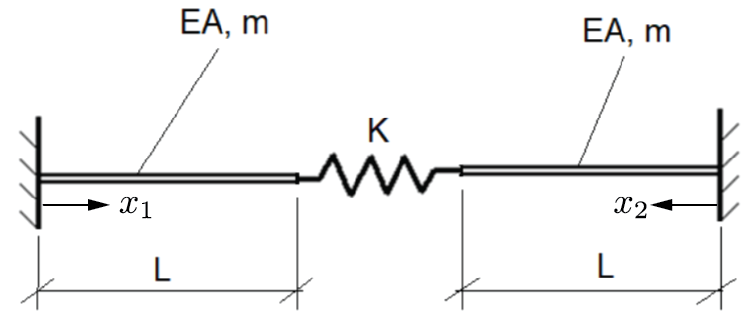
\includegraphics[width=0.5\textwidth]{homework/hw3/assets/hw3_p1.png}
\end{figure}

We define a pair of coordinate systems where coordinates $x_1$ and $x_2$ start from the fixed ends of the two rods, respectively.
This implies that $x_2$ increases in the opposite direction of $x_1$ (one can think of $x_2 = L - x'$ if $x'$ is the reference left end of the right rod).
Define the longitudinal wave speed as $c = \sqrt{EA/m}$, and the displacement field as $u_1(x_1, t)$ and $u_2(x_2, t)$ for the two rods, respectively.
The governing equations and boundary conditions are then 
\begin{equation}
\begin{gathered}
    \frac{\partial^2 u_1}{\partial t^2}(x_1, t) = c^2 \frac{\partial^2 u_1}{\partial x_1^2}(x_1, t), ~~~~ 
    \frac{\partial^2 u_2}{\partial t^2}(x_2, t) = c^2 \frac{\partial^2 u_1}{\partial x_2^2}(x_2, t), \\
    u_1(0, t) = u_2(0, t) = 0, ~~~~ 
    EA \frac{\partial u_1}{\partial x_1}(L, t) = -EA \frac{\partial u_2}{\partial x_2}(L, t) = K \left[ u_2(L, t) - u_1(L, t) \right],
\end{gathered}
\end{equation}
which is the classical wave equation.
The normal mode analysis procedure for this equation was done many times in the previous homework, and is thus not repeated in detail here. 
Let $\omega$ and $\varphi^{(1)}(x_1; \omega), \varphi^{(2)}(x_2; \omega)$ be the eigenmodes (natural frequencies and mode shapes) of the system, where the superscripts are used to distinguish the two rods.
The general solution to the spatial modes are 
\begin{equation}
\begin{aligned}
    \varphi^{(1)}(x_1) &= C^{(1)} \sin \left( \frac{\omega}{c} x_1 \right) + D^{(1)} \cos \left( \frac{\omega}{c} x_1 \right), \\
    \varphi^{(2)}(x_2) &= C^{(2)} \sin \left( \frac{\omega}{c} x_2 \right) + D^{(2)} \cos \left( \frac{\omega}{c} x_2 \right).
\end{aligned}
\end{equation}
subject to boundary conditions 
\begin{equation}
    \varphi^{(1)}(0) = \varphi^{(2)}(0) = 0, ~~~~ EA \frac{d\varphi^{(1)}}{dx_1}(L) = -EA \frac{d\varphi^{(2)}}{dx_2}(L) = K \left[ \varphi^{(2)}(L) - \varphi^{(1)}(L) \right].
\end{equation}
This immediately leads to $D^{(1)} = D^{(2)} = 0$ ($C^{(1)}, C^{(2)} \neq 0$), and 
\begin{equation}\label{eqn:hw3_p1_eigen_bc}
    C^{(1)}\frac{EA\eta}{L} \cos\eta = -C^{(2)}\frac{EA\eta}{L} \cos\eta = K \left[ C^{(2)} - C^{(1)} \right] \sin\eta,
\end{equation}
where we have defined the nondimensional natural frequencies $\eta := \omega L / c$.

From this point, there are two possibilities which we shall discuss separately. 
\begin{enumerate}[(1)]
\item {
    $\cos\eta = 0 ~\Rightarrow ~ \eta_n = (n-1/2)\pi, ~n = 1,2,\ldots$. 
    Since this implies that $\sin\eta \neq 0$, we require $C^{(1)} = C^{(2)}$ rendering the mode shapes on the left and right rods \emph{symmetric}. 
    Here, we have the option to mass-orthonormalize the system by considering the two rods either as a monolithic system or as two separate systems coupled through boundary conditions.
    We choose the latter for this problem, which requires that 
    \begin{equation}\label{eqn:hw3_p1_mass_ortho}
        \int_0^L m \varphi_i^{(1)}(x_1) \varphi_j^{(1)}(x_1) dx_1 = \delta_{ij}, ~~~~ 
        \int_0^L m \varphi_i^{(2)}(x_2) \varphi_j^{(2)}(x_2) dx_2 = \delta_{ij}.
    \end{equation}
    This leads to 
    \begin{equation}\label{eqn:hw3_p1_symm}
    \begin{gathered}
        \varphi_n^{(1)}(x_1) = C_n^{(1)} \sin \left[\left(n - \frac{1}{2}\right)\frac{\pi x_1}{L} \right], ~~~~
        \varphi_n^{(2)}(x_2) = C_n^{(2)} \sin \left[\left(n - \frac{1}{2}\right)\frac{\pi x_2}{L} \right], \\
        C_n^{(1)} = C_n^{(2)} = \sqrt{\frac{2}{mL}}, ~~~~ n = 1, 2, \ldots.
    \end{gathered}
    \end{equation}
}
\item {
    If $\cos\eta \neq 0$, \cref{eqn:hw3_p1_eigen_bc} requires that $C^{(1)} = -C^{(2)} \neq 0$, which corresponds to \emph{antisymmetric} modes.
    It then follows that 
    \begin{equation}\label{eqn:hw3_p1_antisymm_eta}
        \tan\eta = \frac{EA}{2KL}\eta, ~~~~ \eta > 0
    \end{equation}
    which must be solved numerically to yield a countable-infinite number of eigenvalues $\eta_n$. 
    Note that in this equation, $\eta = 0$ is permitted but trivial as it directly leads to zero eigenfunctions.  
    Furthermore, depending on the value of $EA / (2KL)$, there may or may not be an eigenvalue in the interval $(0, \pi/2)$.
    The mass-orthonormality is satisfied similarly by \cref{eqn:hw3_p1_mass_ortho}, which leads to
    \begin{equation}\label{eqn:hw3_p1_antisymm}
    \begin{gathered}
        \varphi_n^{(1)}(x_1) = C_n^{(1)} \sin \left(\eta_n \frac{x_1}{L} \right), ~~~~
        \varphi_n^{(2)}(x_2) = C_n^{(2)} \sin \left(\eta_n \frac{x_2}{L} \right), \\
        C_n^{(1)} = -C_n^{(2)} = {\left[m \int_0^L \sin^2\left(\eta_n \frac{x}{L}\right) dx\right]}^{-\frac{1}{2}}, ~~~~ n = 1, 2, \ldots.
    \end{gathered}
    \end{equation}
    with flexibility on the choice of signs. 
    For completeness, the integral evaluates to 
    \begin{equation}
        \int_0^L \sin^2\left(\eta_n \frac{x}{L}\right) dx = \frac{L}{2}\left[1 - \frac{\sin 2\eta_n}{2\eta_n} \right].
    \end{equation}
}
\end{enumerate}

We now analyze the behavior of the system in the limits $K \rightarrow 0$ and $K \rightarrow \infty$.
Note that since the symmetric modes \cref{eqn:hw3_p1_symm} are unaffected by the spring constant. 
These modes are sine functions ``even'' about the rod ends (think of when $x_1(L)$ and $x_2(L)$ coincides), and collectively form sine functions over both rods between the two fixed ends. 
\emph{In the case of $K \rightarrow \infty$}, \cref{eqn:hw3_p1_antisymm_eta} has no solution in the interval $(0, \pi/2)$, and the solution approaches $\eta_n = n\pi$. 
Concatenating the antisymmetric modes over the two rods forms sine functions between the two fixed ends that are ``odd'' about the rod ends.
Hence, asymptotically the mode shapes reduce to a complete set of sine functions over the entire system, which is identical to the mode shapes of a \emph{fixed-fixed} rod. 
\emph{When $K \rightarrow 0$}, \cref{eqn:hw3_p1_antisymm_eta} is approximated as $\tan\eta \rightarrow\infty$, leading to solutions approaching $\eta_n = (n - 1/2)\pi$ which \emph{coincides with the symmetric modes} (repeated natural frequencies). 
In the limit, the system behaves as if there is no spring connecting the two rods, with both of them vibrating like \emph{fixed-free} rods. 
Effects of the spring connection only manifest at large time scales.

\begin{problem}
    \begin{wrapfigure}{r}{0.45\textwidth}
        \vspace{0.75cm}
        \centering
        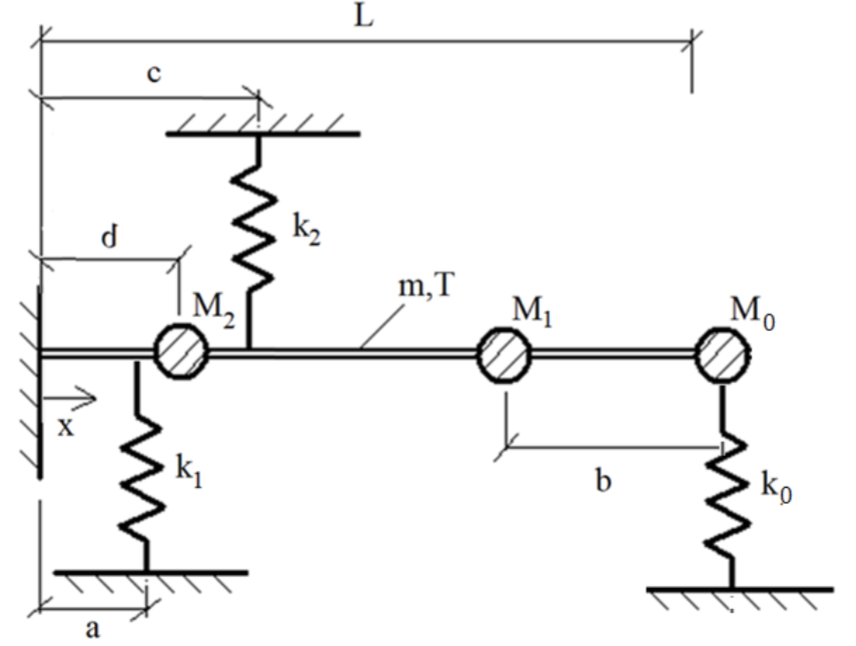
\includegraphics[width=0.95\linewidth]{homework/hw3/assets/hw3_p2.png}
    \end{wrapfigure}
    \textbf{2 (100 pts).} Consider a uniform elastic string undergoing transverse vibration with the grounded vertical springs and the concentrated masses as shown below (disregard gravity). 
    Assign your own numerical values to the system parameters (use reasonable SI units).
    \begin{enumerate}[(i)]
    \item {
        Formulate Rayleigh's quotient for this system and estimate the first natural frequency. 
        Using at least three different test functions perform a convergence study to study the convergence of the Rayleigh quotient to the first natural frequency.
    }
    \item {
        Based on the RQ that you developed in (i) develop a Rayleigh-Ritz methodology for discretizing the eigenvalue problem of this system. 
        Show all steps in detail and using appropriate trial functions compute approximations for the leading three modes of this system.
    }
    \end{enumerate}
\end{problem}

The MATLAB code for this problem can be found at \url{https://github.com/sy-cui/TAM514/blob/main/doc/homework/hw3/assets/hw3_p2.m} and \url{https://github.com/sy-cui/TAM514/blob/main/doc/homework/hw3/assets/hw3_p2_eigen.m}. 
Some other helper functions can be found in the same directory. 
The code is verified to be correct on some simpler problems (e.g.~setting $k_0 = k_1 = k_2 = 0$, $M_0 = M_1 = M_2 = 0$, or leaving one to be nonzero).
\begin{enumerate}[(i)]
\item { % 2(i)
    Let $u(x, t)$ be the transverse displacement of the string, and $\varphi_n(x), \omega_n$ be its $n$-th mode shape and natural frequency, respectively.
    For this linear time-invariant system, if $\tilde{\varphi}_i(x)$ is an approximation of $\varphi_n(x)$, then its Rayleigh quotient can be expressed as the ratio of associated potential and kinetic energy:
    \begin{equation}\label{eqn:hw3_p2_rq}
        \omega_i^2 \approx R[\tilde{\varphi}_i(x)] = \frac{
            k_0 {\tilde{\varphi}_i(L)}^2 + 
            k_1 {\tilde{\varphi}_i(a)}^2 + 
            k_2 {\tilde{\varphi}_i(c)}^2 + 
            \int_0^L T {\tilde{\varphi}'_i(x)}^2 dx 
        }{
            M_0 {\tilde{\varphi}_i(L)}^2 + 
            M_1 {\tilde{\varphi}_i(L-b)}^2 + 
            M_2 {\tilde{\varphi}_i(d)}^2 + 
            \int_0^L m {\tilde{\varphi}_i(x)}^2 dx
        }
    \end{equation}
    Note that the admissable trial functions $\tilde{\varphi}_i(x)$ must still satisfy the fixed boundary condition $\tilde{\varphi}_i(0) = 0$. 
    Next, we need to choose particular $\tilde{\varphi}_i$ for which we can performance convergence study.
    Rather than choosing completely arbitrary functions, we elect to use polynomials of the form $\tilde{\varphi}(x) = \sum_{j=0}^N u_j l_j(\xi(x))$, where $l_j(\xi)$ are Lagrangian polynomials defined with respect to $N+1$ interpolatory nodes $\xi_i$:
    \begin{equation}
        l_j(\xi) = \prod_{\substack{i=0 \\ i\neq j}}^N \frac{\xi - \xi_i}{\xi_j - \xi_i}.
    \end{equation}
    Here, $\xi(x) = (x - L)/2$ is a transformation that maps $x \in [0, L]$ to $\xi \in [-1, 1]$, and hence $l_j(\xi)$ are defined on the interval $[-1, 1]$.
    For simplicity in notation, we define 
    \begin{equation}
        \hat{l}_j(x) = l_j(\xi(x)) = \prod_{\substack{i=0 \\ i\neq j}}^N \frac{\xi(x) - \xi_i}{\xi_j - \xi_i}.
    \end{equation}
    For this problem, we choose \emph{$N = 3$ (4 points)} and the abscissa for the Lagrangian polynomials $\xi_i$ to be Gauss-Legendre-Lobatto points: $\xi_0 = -1$, $\xi_1 = -1/\sqrt{5}$, $\xi_3 = 1/\sqrt{5}$, and $\xi_4 = 1$.
    By convention, we wish to perform all integrals on the unit interval $[-1, 1]$, which implies the use of the Jacobian $J = dx / d\xi = L/2$. 
    Moreover, since $\tilde{\varphi}(x)$ must satisfy the fixed boundary condition on the left end, we require that $u_0 = 0$. 

    After some simple algebra, the Rayleigh quotient of $\tilde{\varphi}(x)$ (\cref{eqn:hw3_p2_rq}) can be expressed as 
    \begin{equation}\label{eqn:hw3_p2_rq_poly}
        R[\tilde{\varphi}(x)] = \frac{\sum_{i,j=0}^3 K_{ij}u_i u_j}{\sum_{i,j=0}^3 M_{ij}u_i u_j},
    \end{equation}
    where 
    \begin{equation}\label{eqn:hw3_p2_KM}
    \begin{aligned}
        K_{ij} &= K_{ji} = k_0 \hat{l}_i(L) \hat{l}_j(L) + k_1 \hat{l}_i(a) \hat{l}_j(a) + k_2 \hat{l}_i(c) \hat{l}_j(c) + \int_{-1}^1 T \frac{dl_i(\xi)}{d\xi} \frac{dl_i(\xi)}{d\xi} \frac{d\xi}{J}, \\
        M_{ij} &= M_{ji} = M_0 \hat{l}_i(L) \hat{l}_j(L) + M_1 \hat{l}_i(L-b) \hat{l}_j(L-b) + M_2 \hat{l}_i(d) \hat{l}_j(d) + \int_{-1}^1 m l_i(\xi) l_j(\xi) J d\xi.
    \end{aligned}
    \end{equation}
    which is readily computable given the material parameters. 
    The integrals can be computed \emph{exactly} using Gauss quadratures by virtual of the integrands being polynomials. 
    Hence, we need only choose the vector $\bv{u} = [u_i] \in \mathbb{R}^4, u_0 = 0$ to construct a polynomial trial function. 
    Based on the lecture, these coefficients $u_1, u_2, u_3$ should be chosen arbitrarily. 
    Here, however, we elect to use a more systematic approach known as the Rayleigh quotient iteration:
    \begin{algorithm}[!ht]
        \caption{Generalized Rayleigh quotient iteration}
        \begin{algorithmic}
        \label{alg:hw3_p2_rq_iter}
        \setlength{\lineskip}{4pt}
        \Require{Stiffness matrix $\bt{K}$, mass matrix $\bt{M}$, initial guess $\bv{u}_0$, number of iterations $k$}
        \Ensure{A natural frequency estimate $\omega$ and the corresponding mass-orthonormalized eigenfunction coefficients $\bv{u}$}
        \State{$\bv{u}_0 \gets \bv{u}_0 / {(\bv{u}_0^T \bt{M} \bv{u}_0)}^{1/2}$}
        \State{$R \gets \bv{u}_0^T \bt{K} \bv{u}_0$}
        \For{$i = 1 : k$}
            \State{$\bv{v} \gets {(\bt{K} - R \bt{M})}^{-1} \bt{M} \bv{u}_{i-1}$}
            \State{$\bv{u}_{i} \gets \bv{v} / {(\bv{v}^T \bt{M} \bv{v})}^{1/2}$}
            \State{$R \gets \bv{u}_i^T \bt{K} \bv{u}_i$}
        \EndFor
        \State{$\omega \gets R$}
        \State{$\bv{u} \gets \bv{u}_k$}
        \end{algorithmic}
    \end{algorithm}

    This algorithm converges \emph{cubically} to the eigenpair that is closest to the initial guess $\bv{u}_0$.
    To find the first natural frequency, we choose $\bv{u}_0 = {[0, 1, 1, 1]}^T$ which is likely to converge to the first eigenfunction.

    For this problem, the material parameters are chosen as shown in \cref{tab:hw3_p2_params}.
    \begin{table}[!ht]
        \centering
        \begin{tabular}{|c|c|c|c|c|c|c|c|}
            \hline
            Parameters & $L$ & $a$ & $b$ & $c$ & $d$ & $m$ & $T$ \\
            \hline
            Values & \qty{1}{\m} & \qty{0.2}{\m} & \qty{0.4}{\m} & \qty{0.4}{\m} & \qty{0.3}{\m} & \qty{30}{\kg\per\m} & \qty{7e3}{\newton} \\
            \hline
            Parameters & $k_0$ & $k_1$ & $k_2$ & $M_0$ & $M_1$ & $M_2$ & \\
            \hline 
            Values & \qty{100}{\newton\per\m} & \qty{200}{\newton\per\m} & \qty{300}{\newton\per\m} & \qty{5}{\kg} & \qty{4}{\kg} & \qty{3}{\kg} &  \\
            \hline
        \end{tabular}
        \caption{Material parameters for Problem 2. }
        \label{tab:hw3_p2_params}
    \end{table}
    The results of the Rayleigh quotient iterations is tabulated in \cref{tab:hw3_p2_rq_results}, and plotted in \cref{tab:hw3_p2_rq_results}.
    The so-called exact results are obtained by using a high-order polynomial ($N = 10$) to approximate the first eigenfunction. 
    This is, of course, not exact as the eigenfunctions are sinusoidal and thus cannot be approximated exactly in the polynomial space. 
    However, based on insights from spectral methods, the numerical error is expected to be small when high polynomial orders are used for this type of Sturm-Liouville problem. 
    As shown in the figures, the eigenpair converges to the first eigenmode rapidly, reaching convergence after only three iterations. 
    However, due to the low polynomial order, the error in the eigenvalue stagnates and cannot be improved further unless better trial functions are used. 
    \begin{table}[!ht]
        \centering
        \begin{tabular}{|c|c|c|c|c|}
            \hline
            Steps & $u_1$ & $u_2$ & $u_3$ & Rayleigh quotient \\
            \hline
            0 & 0.1581 & 0.1581 & 0.1581 & 27.8090 \\
            \hline 
            1 & 0.0737 & 0.1865 & 0.2240 & 19.6589 \\
            \hline 
            2 & 0.0842 & 0.1864 & 0.2144 & 19.4702 \\
            \hline 
            3 & 0.0842 & 0.1864 & 0.2144 & 19.4702 \\
            \hline 
        \end{tabular}
        \caption{Rayleigh quotient iteration results after three iterations with initial guess $\bv{u} = {[0, 1, 1, 1]}^T$ (normalized in the algorithm).}
        \label{tab:hw3_p2_rq_results}
    \end{table}
    \begin{figure}[!ht]
        \centering
        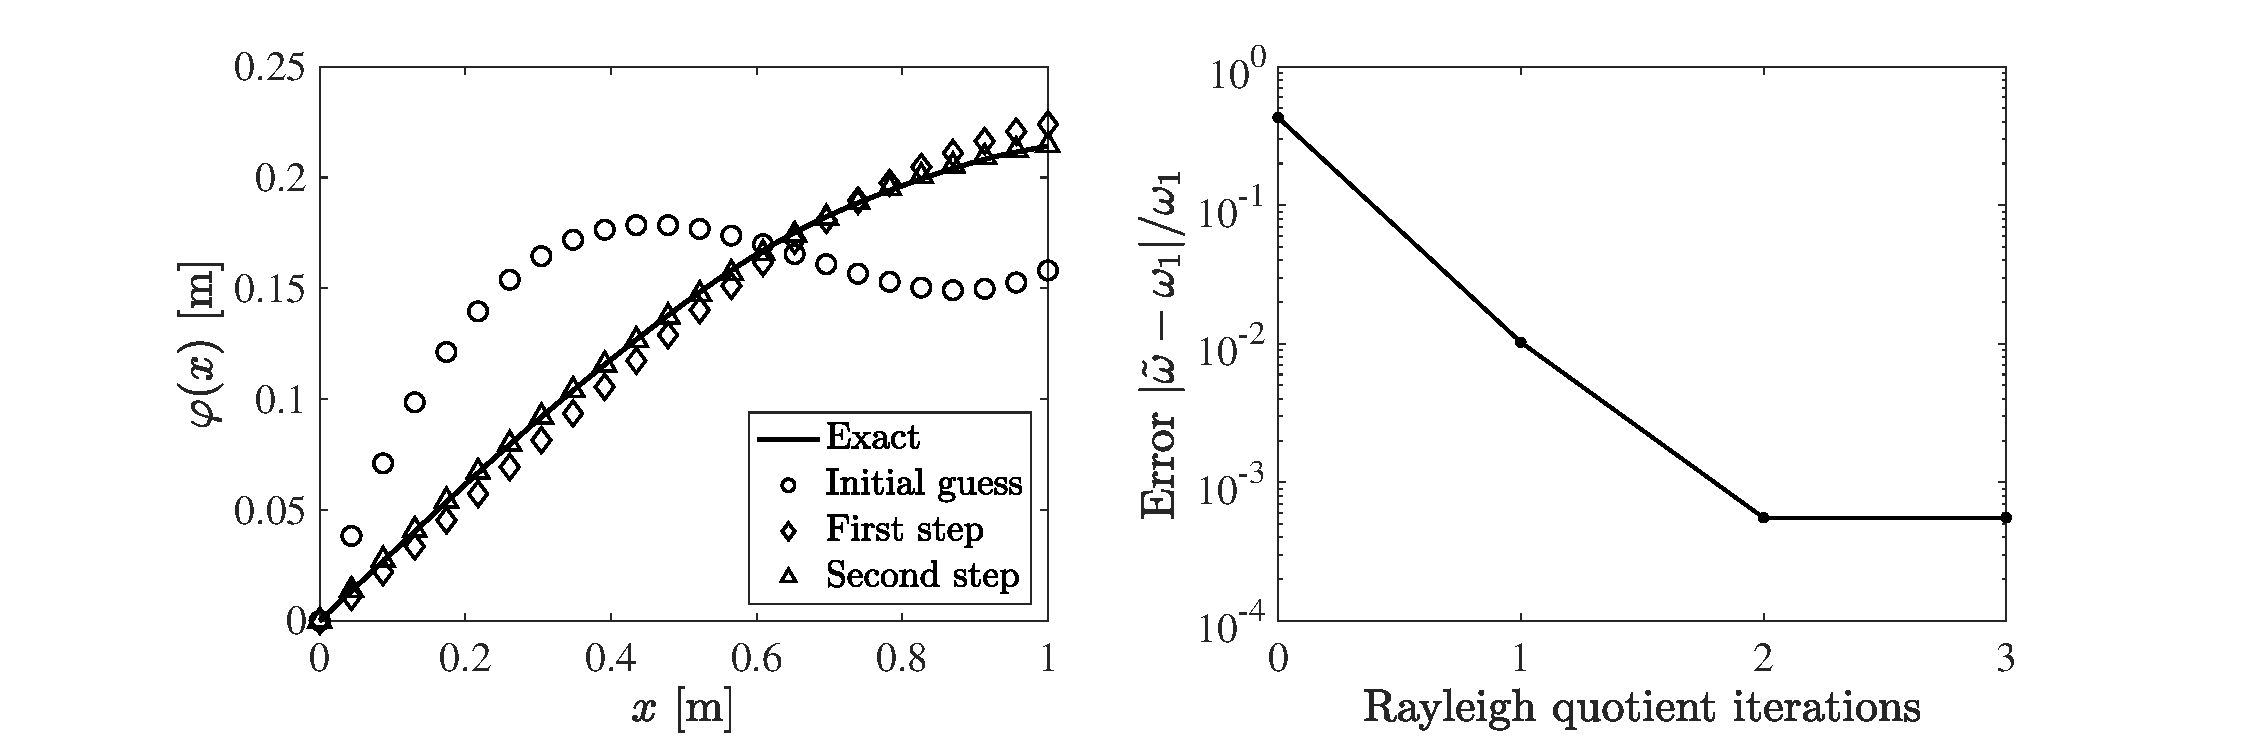
\includegraphics[width=0.9\textwidth]{homework/hw3/assets/hw3_p2_rq.pdf}
        \caption{Rayleigh quotient iteration convergence of the first eigenfunction (left) and eigenvalue (right), compared with the ``exact'' value. 
        The ``exact'' value is obtained by using a high polynomial order ($N = 10$).}
        \label{fig:hw3_p2_rq_results}
    \end{figure}
}
\item { % 2(ii)
    With admissable basis functions readily defined ($l_i(\xi(x))$), the Rayleigh-Ritz eigenvalue problem is formed by finding the stationary points of the Rayleigh quotient \cref{eqn:hw3_p2_rq_poly}:
    \begin{equation}
        0 = \frac{\partial }{\partial u_k} \left(\frac{\sum_{i,j=0}^3 K_{ij} u_i u_j}{\sum_{i,j=0}^3 M_{ij}u_i u_j} \right) = \frac{1}{M_{pq}u_p u_q} \left(K_{ki} u_i - \tilde{\omega}^2 M_{ki}u_i\right)
    \end{equation}
    where we have employed index notation for brevity. 
    Here, $\tilde{\omega}$ is the estimate of the natural frequencies, which is the eigenvalue of the eigenvalue problem $\bt{K}\bv{u} - \tilde{\omega}^2 \bt{M} \bv{u} = 0$ that satisfies $u_0 = 0$. 
    Note that $\bt{K}$ and $\bv{M}$ are readily defined in \cref{eqn:hw3_p2_KM}, except now we are directly solving the full eigenproblem rather than using Rayleigh quotient to find a specific eigenvalue. 
    Using the same material parameters as in \cref{tab:hw3_p2_params} and $N = 3$, the leading three approximated eigenpairs are tabulated in \cref{tab:hw3_p2_rr_results}.
    The eigenfunctions are further plotted in \cref{fig:hw3_p2_rr_results}. 
    Note that the first mode is the same as the one obtained from the Rayleigh quotient iteration.
    \begin{table}[!ht]
        \centering
        \begin{tabular}{|c|c|c|c|c|}
            \hline
            Index & $u_1$ & $u_2$ & $u_3$ & Eigenvalue \\
            \hline 
            1 & 0.0842 & 0.1864 & 0.2145 & 19.4702 \\
            \hline 
            2 & -0.1986 & -0.0091 & 0.2188 & 58.1247 \\
            \hline 
            3 & 0.1700 & -0.2051 & 0.2166 & 104.9341 \\
            \hline 
        \end{tabular}
        \caption{Rayleigh-Ritz approximation of the first three eigenpairs using $N = 3$. }
        \label{tab:hw3_p2_rr_results}
    \end{table}
    \begin{figure}[!ht]
        \centering
        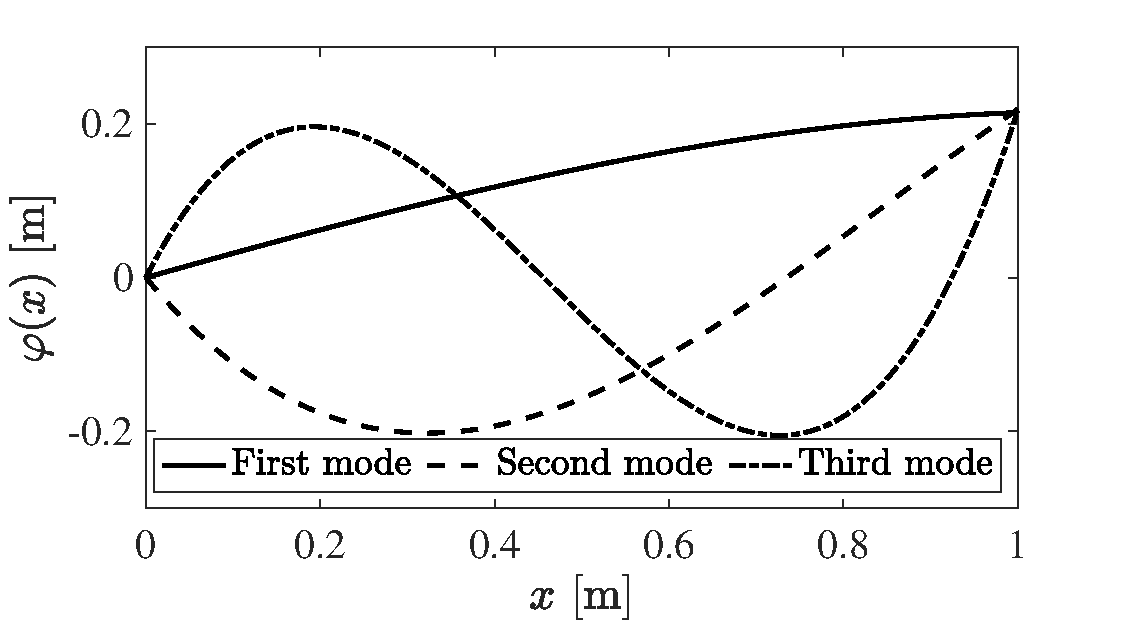
\includegraphics[width=0.52\textwidth]{homework/hw3/assets/hw3_p2_rr.pdf}
        \caption{Rayleigh-Ritz approximation of the first three eigenfunctions.}
        \label{fig:hw3_p2_rr_results}
    \end{figure}
}
\end{enumerate}

\newpage
\begin{problem}
    \textbf{3 (100 pts).} Consider the following nonuniform rod in axial vibration, with elastic and inertial properties $EA(x)$ and $m(x)$ varying as:
    \begin{equation}
        EA(x) = EA\left[1 - \sin^{3/2}(0.5x/L) \right], ~~~~ m(x) = m\left[1 - \sin^{3/2}(0.5x/L) \right]
    \end{equation}
    Use the Rayleigh-Ritz method to approximate the leading three normal modes of this system.
    Assume a steel rod with $L=\qty{1}{\m}$. 
    Compare your results with the first three normal modes of the uniform rod with properties $EA(x) = EA$ and $m(x) = m$. 
    Do the differences make sense? 
    Justify the differences using mechanics arguments.  
\end{problem}
\begin{figure}[!ht]
    \centering
    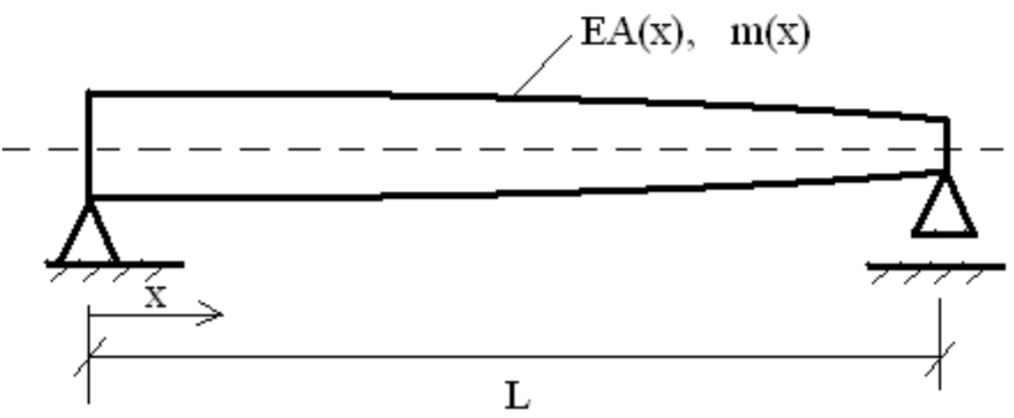
\includegraphics[width=0.5\textwidth]{homework/hw3/assets/hw3_p3.png}
\end{figure}

MATLAB code for this problem can be found at \url{https://github.com/sy-cui/TAM514/blob/main/doc/homework/hw3/assets/hw3_p3.m}.

We follow the same methodology as in Problem 2, where we form the discretized eigenvalue problem $\bt{K} \bv{u} = \tilde{\omega}^2 \bt{M} \bv{u}$. 
The same Lagrangian basis functions are used with the abscissa chosen to be $N + 1$ Gauss-Legendre-Lobatto points (polynomial order $N + 1$). 
The stiffness and mass matrices are 
\begin{equation}
\begin{aligned}
    K_{ij} &= K_{ji} = \int_0^L EA(x) \frac{dl_i(\xi)}{d\xi} \frac{dl_j(\xi)}{d\xi} J d\xi, \\
    M_{ij} &= M_{ji} = \int_0^L m(x) l_i(\xi) l_j(\xi) J d\xi,
\end{aligned}
\end{equation}
computed numerically using quadratures. 
Granted, the integrands are not polynomials and hence the Gauss quadrature is unable to integrate exactly. 
Nonetheless, a high-order ($\sim 2N$) Gauss-Legendre quadrature is used in the code to minimize the errors incurred by integration, which should ensure that the error is dominated by the choice of finite-dimensional basis functions rather than numerical integration. 

For this problem, we choose the material properties to be close to an aluminum rod that has 
\begin{equation}
    E = \qty{70}{\giga\pascal}, ~~~~ A = \qty{0.01}{\m\squared}, ~~~~ \rho = \qty{2700}{\kg\per\m\cubed}, ~~~~ L = \qty{1}{\m}.
\end{equation}
Moreover, we use a basis polynomial order $N = 8$. 
At this order, the code is verified to yield next to negligible error if $EA(x) = EA$ and $m(x) = m$.
MATLAB's native eigenvalue routine is used to solve the generalized eigenvalue problem, which is of size $N \times N$ given that the left end is fixed. 
The lowest three eigenvalues, along with their corresponding mass-orthonormalized eigenfunctions, are tabulated in \cref{tab:hw3_p3_results}. 
Note that $u_0 = 0$ due to the fixed boundary condition. 
\begin{table}[!ht]
    \centering
    \begin{tabular}{|c|c|c|c|c|c|c|c|c|c|}
        \hline
        Index & Eigenvalue & $u_1$ & $u_2$ & $u_3$ & $u_4$ & $u_5$ & $u_6$ & $u_7$ & $u_8$ \\
        \hline 
        1 & 867.07 & 0.0230 & 0.0738 & 0.1427 & 0.2134 & 0.2686 & 0.2992 & 0.3093 & 0.3105 \\
        \hline 
        2 & 2422.9 & 0.0644 & 0.1909 & 0.2787 & 0.1961 & -0.0362 & -0.2403 & -0.3206 & -0.3298 \\
        \hline 
        3 & 4013.0 & 0.1050 & 0.2628 & 0.1639 & -0.2096 & -0.2368 & 0.1053 & 0.3066 & 0.3319 \\
        \hline 
    \end{tabular}
    \caption{Rayleigh-Ritz approximation of the first three eigenpairs using $N = 8$. }
    \label{tab:hw3_p3_results}
\end{table}

If $EA(x) = EA$ and $m(x) = m$, we have 
\begin{equation}
    \omega_n = \left(n + \frac{1}{2}\right)\frac{\pi c}{L}, ~~~~ \varphi_i(x) = \sqrt{\frac{2}{m L}} \sin \left(\frac{\omega_n}{c} x\right), ~~~~ c = \sqrt{\frac{EA}{m}}.
\end{equation}
With the assumed material parameters, the first three eigenfunctions in both cases are plotted in \cref{fig:hw3_p3_results}.
It is observed that for small $x$, the eigenfunctions of the nonuniform rod is close to the uniform rod.
This consistency is not preserved for larger $x$, where the eigenfunctions show significant disagreement.
This is expected as the nonuniformity arises from the function
\begin{equation}\label{eqn:hw3_p3_fx}
    f(x) = 1 - \sin^{3/2}\left(\frac{x}{2L}\right), ~~~~ f'(x) = -\frac{3}{4L} \sin^{1/2}\left(\frac{x}{2L}\right) \cos\left(\frac{x}{2L}\right),
\end{equation}
which is plotted in \cref{fig:hw3_p3_fx}.
Note that for small $x$, $f(x)$ is close to 1, which means $EA(x) \approx EA$ and $m(x) \approx m$. 
Moreover, $f'(x)$ is close to zero in this range, suggesting that $f(x)$ does not deviates from 1 rapidly. 
This leads to the eigenfunctions of the nonuniform rod being close to that of the uniform rod for small $x$. 
As $x \rightarrow L$, there is significant deviation of $EA(x)$ and $m(x)$ from their uniform values, leading to the eigenfunctions being different. 
\begin{figure}[!ht]
    \centering
    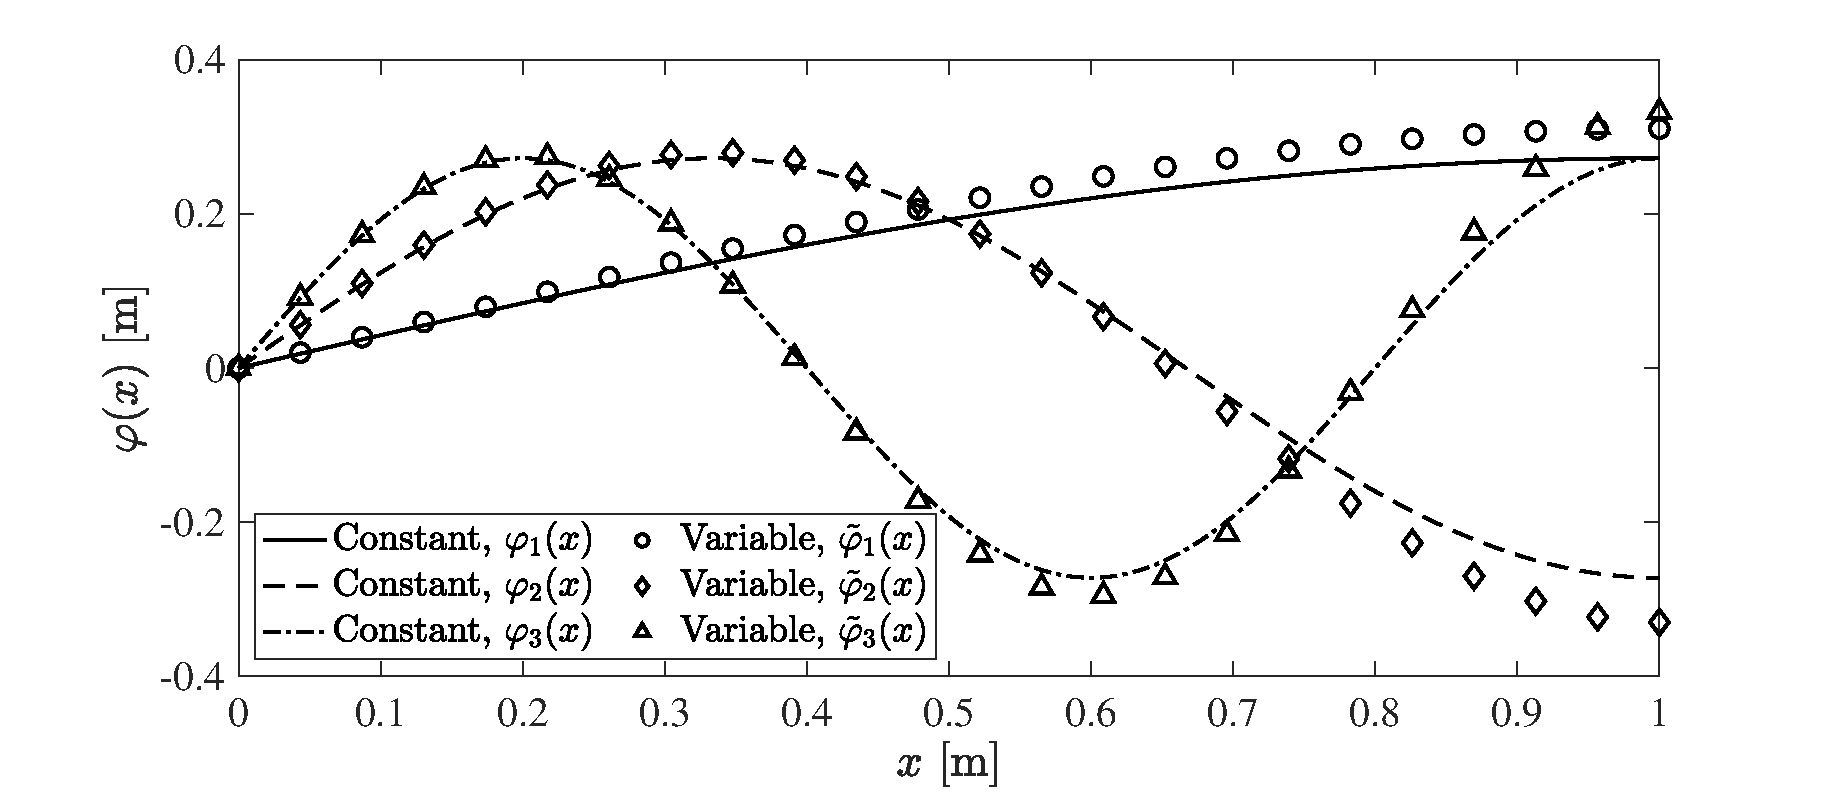
\includegraphics[width=\textwidth]{homework/hw3/assets/hw3_p3_result.pdf}
    \caption{Comparison of the first three eigenfunctions of the nonuniform rod (numerical) with the uniform rod (analytical). 
    ``Constant'' and ``variable'' refer to the nature of $EA(x)$ and $m(x)$, with the former representing the uniform rod and the latter the nonuniform rod.}
    \label{fig:hw3_p3_results}
\end{figure}
\begin{figure}[!ht]
    \centering
    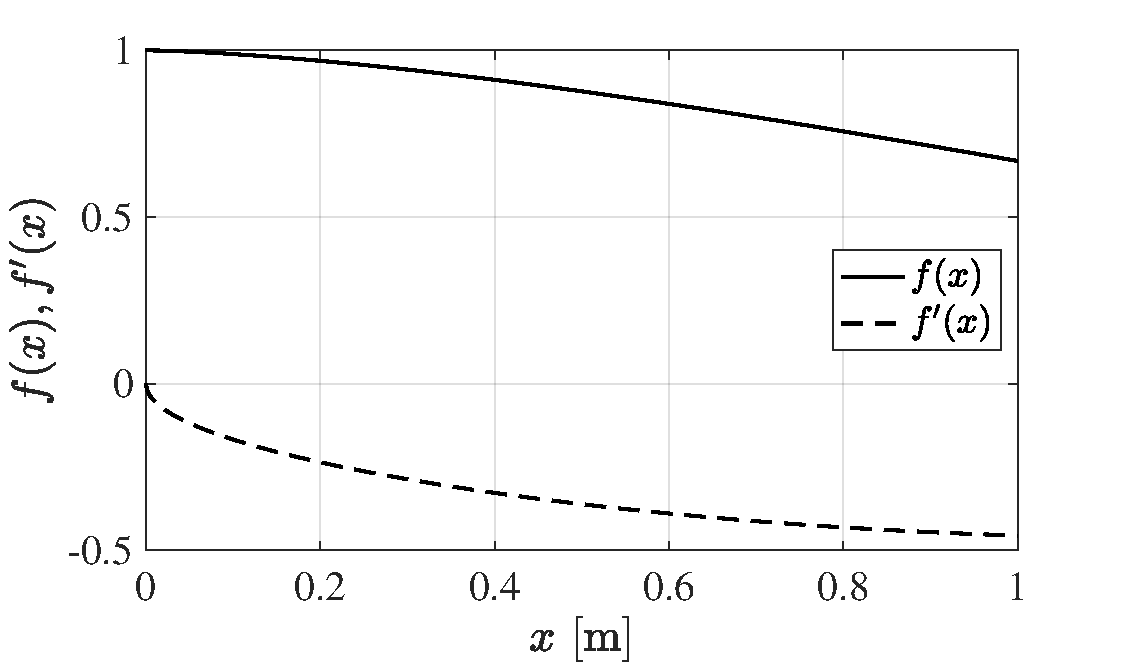
\includegraphics[width=0.6\textwidth]{homework/hw3/assets/hw3_p3_fx.pdf}
    \caption{The profile function $f(x)$ and its derivative $f'(x)$ (\cref{eqn:hw3_p3_fx}).}
    \label{fig:hw3_p3_fx}
\end{figure}

\newpage
\begin{problem}
    \textbf{4 (100 points)}. Consider the following (normalized) elastic string undergoing transverse vibrations governed by teh classical wave equation:
    \begin{equation}
        \frac{\partial^2 u(x, t)}{\partial t^2} = \frac{\partial^2 u(x, t)}{\partial x^2}, ~~ u(x, 0) = 0, ~~ \frac{\partial u(x, 0)}{\partial t} = 0, ~~ 0 \leq x \leq 1, ~~ t \geq 0.
    \end{equation}
    The string has fixed-fixed supports which undergo prescribed motions as follows:
    \begin{equation}
        u(0, t) = u_{g_1}(t) \equiv 2(1 - \cos \omega t), ~~~~ u(1, t) = u_{g_2}(t) \equiv \cos (2\omega t) - 1, ~~~~ t \geq 0.
    \end{equation}
    Compute the transverse vibrations of the string. Can resonance occur in this system? If yes, under what condition(s) can this occur?
\end{problem}
We decompose the solution into a quasi-steady and a transient part:
\begin{equation}
    u(x, t) = \bar{u}(x, t) + \tilde{u}(x, t),
\end{equation}
where $\bar{u}(x, t)$ satisfy the boundary conditions at every $t$, and follows a linear relation everywhere in between:
\begin{equation}\label{eqn:hw3_p4_bar_u}
    \bar{u}(x, t) = (1 - x) u_{g_1}(t) + x u_{g_2}(t) = \left[\cos(2\omega t) + 2\cos\omega t - 3\right] x + 2 - 2\cos\omega t.
\end{equation}
This ensures that $\tilde{u}(x, t)$ satisfy the homogeneous Dirichlet boundary conditions at all time: $\tilde{u}(0, t) = \tilde{u}(1, t) = 0$. 
The initial conditions on $\tilde{u}(x, t)$ are 
\begin{equation}
    \tilde{u}(x, 0) = u(x, 0) - \bar{u}(x, 0) = 0, ~~~~ \frac{\partial \tilde{u}(x, 0)}{\partial t} = \frac{\partial u(x, 0)}{\partial t} - \frac{\partial \bar{u}(x, 0)}{\partial t} = 0.
\end{equation}
We can now perform normal mode analysis on $\tilde{u}(x, t)$ which satisfy the forced wave equation 
\begin{equation}
    \frac{\partial^2 \tilde{u}(x, t)}{\partial t^2} = \frac{\partial^2 \tilde{u}(x, t)}{\partial x^2} - \frac{\partial^2 \bar{u}(x, t)}{\partial t^2} = \frac{\partial^2 \tilde{u}(x, t)}{\partial x^2} + \underbrace{2\omega^2 \left[(2\cos2\omega t + \cos\omega t) x - \cos\omega t \right]}_{f(x, t)},
\end{equation}
where $f(x, t)$ is a forcing term induced by the time-dependent Dirichlet boundary conditions. 
With the ansatz $\tilde{u}(x, t) = \varphi(x) \eta(t)$ under fixed-fixed conditions, the normal mode analysis yields 
\begin{equation}\label{eqn:hw3_p4_spatial_soln}
    \varphi_n(x) = \sqrt{2}\sin(\tilde{\omega}_n x), ~~~~ \tilde{\omega}_n = n\pi, ~~~~ n = 1, 2, \ldots,
\end{equation}
where $\tilde{\omega}_n$ are the natural frequencies. 
The constant coefficient is chosen such that mass-orthonormality is satisfied, i.e., $\int_0^1 \varphi_i(x) \varphi_j(x) dx = \delta_{ij}$.
Each temporal mode is governed by the equation 
\begin{equation}\label{eqn:hw3_p4_temporal_ode}
\begin{aligned}
    \ddot{\eta}_n(t) + \eta_n(t) &= \int_0^1 f(x, t) \varphi_n(x) dx, ~~~~ n = 1, 2, \ldots \\
    &= -\frac{2\sqrt{2} \omega^2}{n\pi} [\cos\omega t + 2{(-1)}^n \cos2\omega t]
\end{aligned}
\end{equation}
subject to initial conditions 
\begin{equation}\label{eqn:hw3_p4_temporal_bc}
    \eta_n(0) = 0, ~~~~ \dot{\eta}_n(0) = 0.
\end{equation}
Obviously, resonance \emph{can occur when $\omega = 1$ or $\omega = 0.5$}.
If resonance does not occur ($\omega \neq 1, 0.5$), solving \cref{eqn:hw3_p4_temporal_ode,eqn:hw3_p4_temporal_bc} yields 
\begin{equation}\label{eqn:hw3_p4_temporal_soln_no_resonance}
    \eta_n(t) = \frac{2\sqrt{2}\omega^2}{n\pi}\left[\frac{1}{1-\omega^2}(\cos t - \cos\omega t) + \frac{2{(-1)}^n}{1 - 4\omega^2}(\cos t - \cos 2 \omega t) \right]
\end{equation}
If $\omega = 1$, the resonance solution is 
\begin{equation}\label{eqn:hw3_p4_temporal_soln_resonance_1}
    \eta_n(t) = -\frac{\sqrt{2}}{n\pi}\left[t\sin t + \frac{4{(-1)}^n}{3}(\cos t - \cos 2 t) \right].
\end{equation}
If $\omega = 0.5$, the resonance solution is 
\begin{equation}\label{eqn:hw3_p4_temporal_soln_resonance_2}
    \eta_n(t) = \frac{\sqrt{2}}{2n\pi}\left[\frac{4}{3}\left(\cos t - 2\cos \frac{t}{2}\right) + {(-1)}^n t\sin t \right].
\end{equation}
The final solution is 
\begin{equation}
    u(x, t) = \bar{u}(x, t) + \sum_{n=1}^\infty \varphi_n(x) \eta_n(t).
\end{equation}
with $\bar{u}(x, t)$, $\varphi_n(x)$, and $\eta_n(t)$ given in \cref{eqn:hw3_p4_bar_u,eqn:hw3_p4_spatial_soln,eqn:hw3_p4_temporal_soln_no_resonance,eqn:hw3_p4_temporal_soln_resonance_1,eqn:hw3_p4_temporal_soln_resonance_2}. 

\begin{problem}
    \textbf{5 (100 points)}. We reconsider problem 5 of HW2. Assign reasonable numerical values to the system parameters in SI units.
    \begin{enumerate}[(i)]
        \item {
            Compute the fundamental natural frequency and the corresponding first eigenfunction by (numerically) solving the exact eigenvalue problem.
        } 
        \item {
            Provide three different estimates for the fundamental natural frequency using Rayleigh's quotient and compare them with the exact value. 
            In each case the test function that you will use approximates the first eigenfunction, so compare the approximations of approximate eigenfunctions with exact first eigenfunction as well.
        }
    \end{enumerate}
\end{problem}
\begin{figure}[!ht]
    \centering
    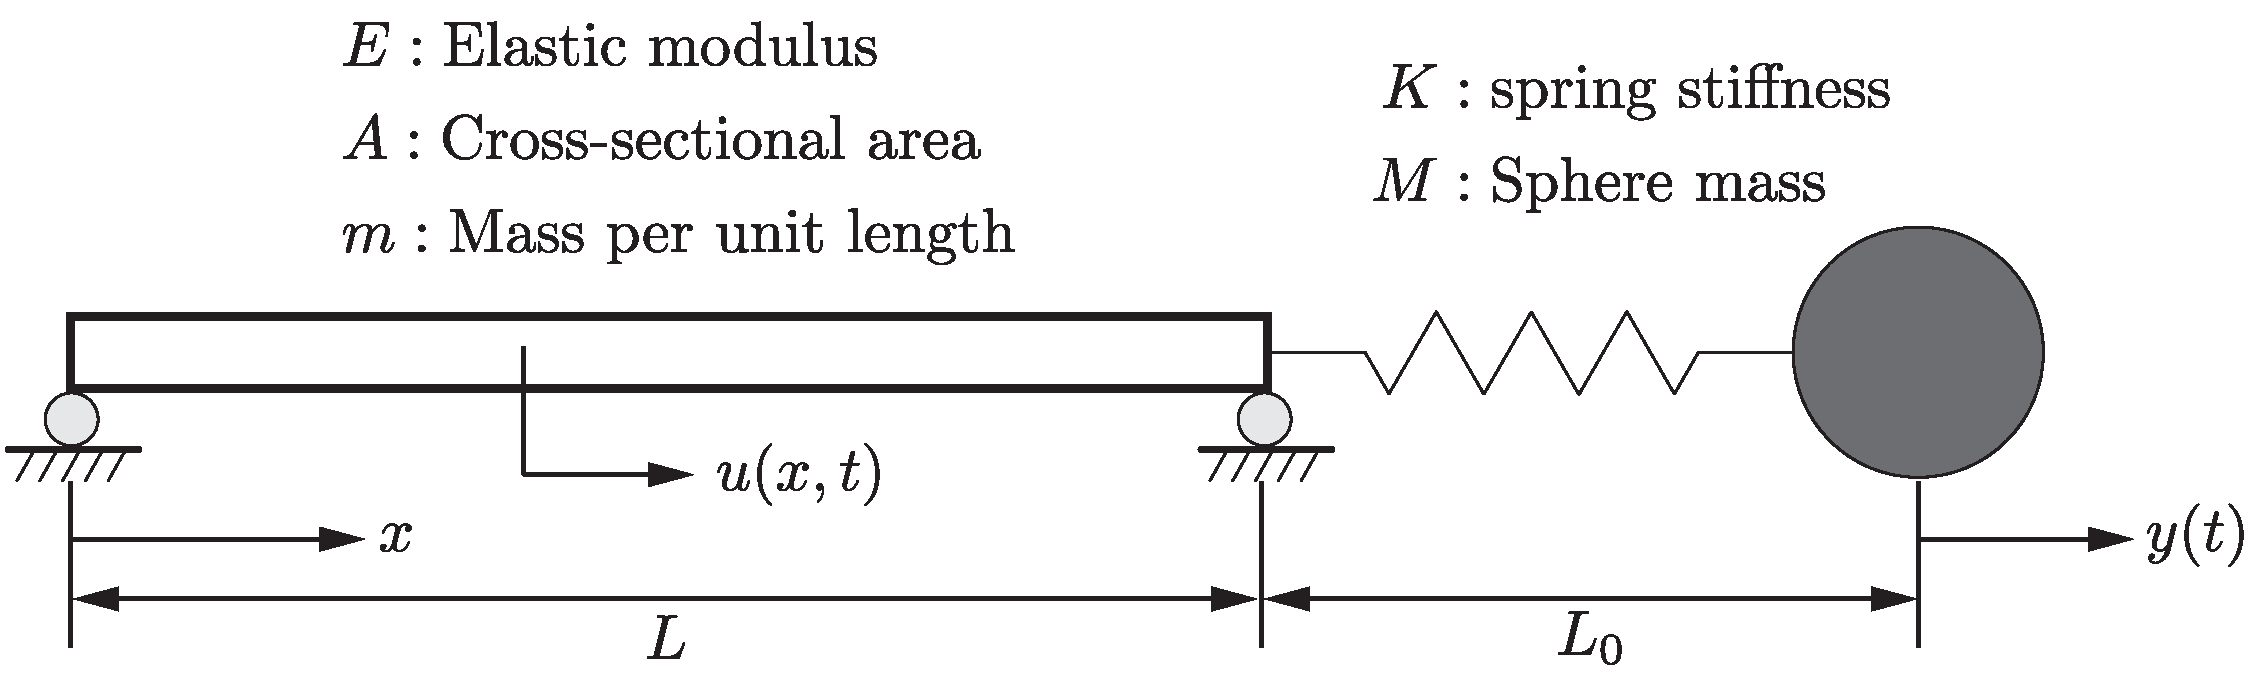
\includegraphics[width=0.8\textwidth]{homework/hw3/assets/hw3_p5.pdf}
\end{figure}

MATLAB code for this problem can be found at \url{https://github.com/sy-cui/TAM514/blob/main/doc/homework/hw3/assets/hw3_p5.m}.

\begin{enumerate}[(i)]
\item {
    For this problem, we conduct normal mode analysis with the ansatz 
    \begin{equation}
        u(x, t) = \sum_{i=0}^\infty \varphi_i(x) \eta_i(t), ~~~~ y(t) = \sum_{i=0}^\infty \psi_i \eta_i(t)
    \end{equation}
    where the following is satisfied:
    \begin{equation}\label{eqn:hw3_p5_eigenproblem}
        EA \varphi_i''(x) + \omega_i^2 m \varphi_i(x) = 0, ~~~~ \eta_i''(t) + \omega_i^2 \eta_i(t) = 0.
    \end{equation}
    The boundary condition for the rod, along with the equation of motion of the mass, read 
    \begin{equation}\label{eqn:hw3_p5_bc_1}
        \varphi_i'(0) = 0, ~~~~ EA \varphi_i'(L) - K(\psi_i - \varphi_i(L)) = 0, ~~~~ (K - \omega_i^2 M) \psi_i - K\varphi_i(L) = 0.
    \end{equation}
    The last two relations reveal the following
    \begin{equation}\label{eqn:hw3_p5_bc_2}
        \psi_i = \frac{K}{K - \omega_i^2 M} \varphi_i(L), ~~~~ \frac{\omega_i^2 KM}{K - \omega_i^2 M} \varphi_i(L) = EA \varphi_i'(L),
    \end{equation}
    wherein the latter, along with $\varphi_i'(0) = 0$, can be used to solve the eigenvalue problem \cref{eqn:hw3_p5_eigenproblem}:
    \begin{equation}\label{eqn:hw3_p5_eigenfunction}
        \boxed{\varphi_i(x) = C_i \cos\left(\eta_i \frac{x}{L}\right), ~~~~ \eta_i = \omega_i L \sqrt{\frac{m}{EA}}}.
    \end{equation}
    where the nondimensional natural frequencies $\eta_i$ satisfies the following 
    \begin{equation}\label{eqn:hw3_p5_eval_eqn}
        \tan \eta_i = - \left(\frac{KL}{EA}\right) \frac{\eta_i}{\Omega^2 - \eta_i^2}, ~~~~ \Omega^2 = \frac{mKL^2}{MEA}
    \end{equation}
    where $\Omega$ is a nondimensional frequency associated with the coupling between the continuum and discrete mass. 
    The mass-orthonormality condition can be obtained by taking the inner product of the spatial eigenvalue problem \cref{eqn:hw3_p5_eigenproblem} with $\varphi_j(x)$ and integrating by parts twice. 
    The result reads 
    \begin{equation}\label{eqn:hw3_p5_mass_orthonormality}
        \int_0^L m \varphi_i(x) \varphi_j(x) dx + \frac{K^2M \varphi_i(L) \varphi_j(L)}{(K - \omega_i^2 M)(K - \omega_j^2 M)} = \delta_{ij}.
    \end{equation}   
    
    The following parameters are assumed:
    \begin{equation}
        E = \qty{70}{\giga\pascal}, ~~~~ A = \qty{0.01}{\m\squared}, ~~~~ m = \qty{27}{\kg\per\m}, ~~~~ L = \qty{1}{\m}, ~~~~ K = \qty{e7}{\newton\per\m}, ~~~~ M = \qty{10}{\kg}
    \end{equation}
    We remark that \cref{eqn:hw3_p5_eval_eqn} does not preclude the rigid body mode $\omega_0 = \qty{0}{\radian\per\s}$, since the system is not constrained.
    Here, however, we wish to find the first (non-zero) natural frequency and its corresponding eigenfunction.
    By solving \cref{eqn:hw3_p5_eval_eqn} numerically for its first root, we find $\eta_1 = 1.8026$, and $\boxed{\omega_1 = \qty{917.8330}{\radian\per\s}}$.
    To find the mass-orthonormalized eigenfunction, we substitute \cref{eqn:hw3_p5_eigenfunction} into \cref{eqn:hw3_p5_mass_orthonormality} to obtain 
    \begin{equation}
        \boxed{C_1 = {\left[\frac{mL}{2}\left(1 + \frac{\sin 2\eta_1}{2\eta_1}\right) + \frac{K^2 M \cos^2 \eta_1}{{(K-\omega_1^2 M)}^2}\right]}^{-\frac{1}{2}} \approx \qty{0.1739}{\kg^{-1/2}}}. 
    \end{equation} 
    The graphical representation of the first nondimensional eigenvalue $\eta_1$ as the intersection of both sides of \cref{eqn:hw3_p5_eval_eqn} is show in \cref{fig:hw3_p5_intersect}.
    \begin{figure}[!ht]
        \centering
        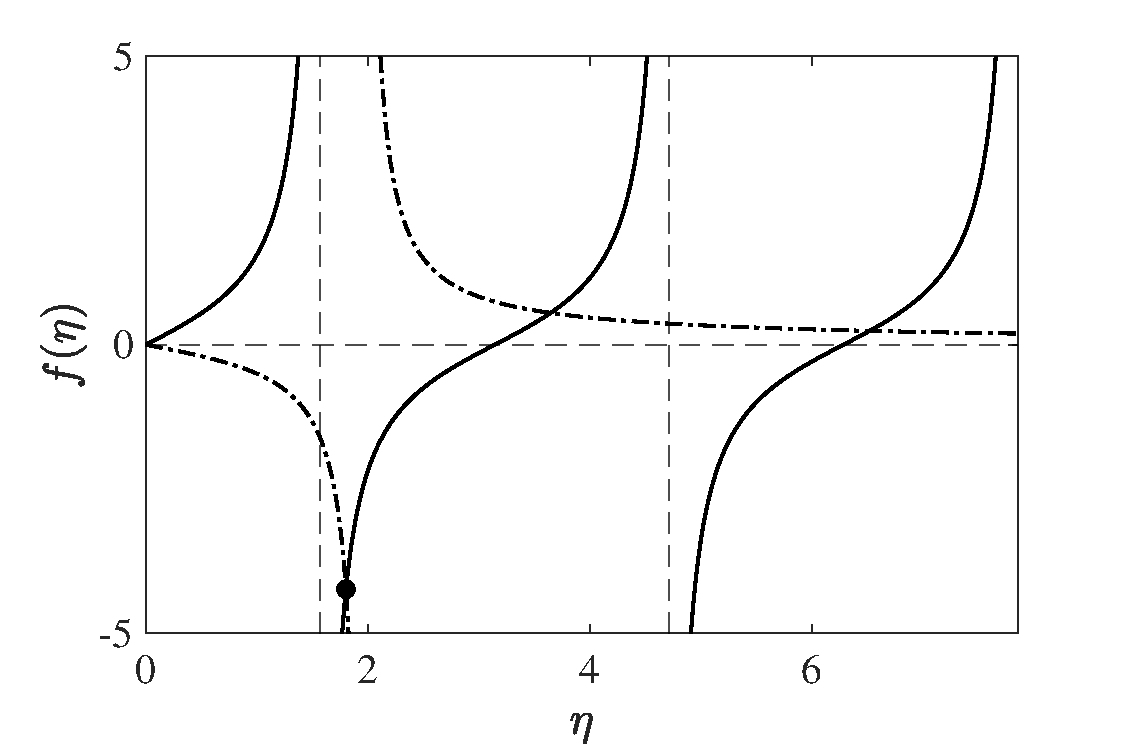
\includegraphics[width=0.6\textwidth]{homework/hw3/assets/hw3_p5_intersect.pdf}
        \caption{Graphical representation of the first nondimensional eigenvalue $\eta_1$ as the intersection of both sides of \cref{eqn:hw3_p5_eval_eqn}. 
        The left- and right-hand-side functions are plotted in solid and dot-dash lines, respectively. 
        The first eigenvalue $\eta_1 = 1.8026$ is highlighted.}
        \label{fig:hw3_p5_intersect}
    \end{figure}
    
}
\item {
    Given a pair of trial ``functions'' ($\tilde{\varphi}(x), \tilde{\psi})$ that presumably satisfy the boundary conditions \cref{eqn:hw3_p5_bc_1}, its Rayleigh quotient associated with this system is obtained by substituting it into \cref{eqn:hw3_p5_eigenproblem}.
    Note that even though $\tilde{\psi}$ is only a scalar, it still needs to be included in the trial functions, and hence the second equation \cref{eqn:hw3_p5_bc_1} should be regarded as its equation of motion. 
    Suppose that it yields an approximate eigenvalue $\tilde{\omega}^2$.
    Taking \cref{eqn:hw3_p5_eigenproblem}'s inner product with $\tilde{\varphi}(x)$ then leads to 
    \begin{equation}\label{eqn:hw3_p5_rq_1}
    \begin{aligned}
        0 &= \int_0^L EA \tilde{\varphi}''(x) \tilde{\varphi}(x) dx + \tilde{\omega}^2 \int_0^L m {\tilde{\varphi}(x)}^2 dx \\
        &= {\left[EA \tilde{\varphi}'(x) \tilde{\varphi}(x) \right]}_0^L - \int_0^L EA {\tilde{\varphi}'(x)}^2 dx + \tilde{\omega}^2 \int_0^L m {\tilde{\varphi}(x)}^2 dx \\
        &= K\tilde{\varphi}(L)[\tilde{\psi} - \tilde{\varphi}(L)]- \int_0^L EA {\tilde{\varphi}'(x)}^2 dx + \tilde{\omega}^2 \int_0^L m {\tilde{\varphi}(x)}^2 dx
    \end{aligned}
    \end{equation}
    where we have used the second equation of \cref{eqn:hw3_p5_bc_1}. 
    This is complemented by the the ``equation of motion'' for $\tilde{\psi}$:
    \begin{equation}\label{eqn:hw3_p5_rq_2}
        \tilde{\omega}^2 M \tilde{\psi}^2 + K\tilde{\psi}(\tilde{\varphi}(L) - \tilde{\psi}) = 0.
    \end{equation}
    which has been multiplied by $\tilde{\psi}$ to obtain the quadratic, energy-like form. 
    Adding \cref{eqn:hw3_p5_rq_1,eqn:hw3_p5_rq_2} and rearranging yields the Rayleigh quotient:
    \begin{equation}\label{eqn:hw3_p5_rq}
        \boxed{\tilde{\omega}^2 = R[\tilde{\varphi}(x), \tilde{\psi}] = \frac{K{\left[\tilde{\varphi}(L) - \tilde{\psi}\right]}^2 + \int_0^L EA {\tilde{\varphi}'(x)}^2 dx}{M \tilde{\psi}^2 + \int_0^L m {\tilde{\varphi}(x)}^2}}
    \end{equation}

    Next, we need a number of \emph{admissable} trial functions $(\tilde{\varphi}(x), \tilde{\psi})$ to substitute into the Rayleigh quotient \cref{eqn:hw3_p5_rq}.
    We adopt the same spectral approach as in Problem 2, where we let $\tilde{\varphi}(x) = \sum_{j=0}^N u_j l_j(\xi(x))$, where $\xi(x) = x/L - 1$ and $l_j(\xi)$ are the Lagrangian polynomials defined on the interval $[-1, 1]$ with respect to $N + 1$ Gauss-Legendre-Lobatto points.
    In addition, $\tilde{\psi}$ is chosen as a random scalar that is regarded as an independent variable. 
    Hence, the stiffness and mass matrices ($\bt{K}$, $\bt{M}$) will be of dimension $(N+2)\times(N+2)$ ($N+1$ Lagrangian interpolants and $\tilde{\psi}$).
    For this problem, we choose \emph{$N = 8$}. 

    Let $\hat{\bv{e}}_j$ be the $j$-th canonical basis (column vector) in $\mathbb{R}^{N+1}$, defined as $\hat{e}_{j,i} = \delta_{ij}, ~i,j=0, \ldots, N$. 
    Furthermore, let $J = dx/d\xi = L/2$ be the Jacobian, which then leads to 
    \begin{equation}
    \begin{gathered}
        \bt{K} = \begin{bmatrix}
            \bt{K}_{11} & \bt{K}_{12} \\
            \bt{K}_{21} & \bt{K}_{22}
        \end{bmatrix},  \\
        \bt{K}_{11} = \left[\int_{-1}^1 EA \frac{d l_i(\xi)}{d\xi} \frac{d l_j(\xi)}{d\xi}\frac{d\xi}{J}  \right]  + K\hat{\bv{e}}_{N} \otimes \hat{\bv{e}}_{N}, ~~~~ K_{12} = K_{21}^T = -K \hat{\bv{e}}_{N}, ~~~~ K_{22} = [K], \\
        \bt{M} = \begin{bmatrix}
            \bt{M}_{11} & \bt{M}_{12} \\
            \bt{M}_{21} & \bt{M}_{22}
        \end{bmatrix},  \\
        \bt{M}_{11} = \left[\int_{-1}^1 m l_i(\xi) l_j(\xi) J d\xi  \right], ~~~~ M_{12} = M_{21}^T = \bv{0}, ~~~~ M_{22} = [M].
    \end{gathered}
    \end{equation}
    This essentially leads to the discretized eigenvalue problem $\bt{K}\bv{u} = \tilde{\omega}^2 \bt{M} \bv{u}$, where $\bv{u}$ is defined as 
    \begin{equation}
        \bv{u} := {[u_0, \ldots, u_N, \tilde{\psi}]}^T.
    \end{equation}
    To use the Rayleigh quotient approach to find the fundamental frequency, we incur the Rayleigh quotient iteration \cref{alg:hw3_p2_rq_iter} with an \emph{non-normalized initial guess interpolating the first eigenfunction of the free-fixed rod}:
    \begin{equation}
        u_i = \cos\left(\frac{\pi L}{4}(\xi_i + 1)\right), ~~ i = 0, \ldots, N=8, ~~~~ \tilde{\psi} = 0.
    \end{equation}
    Results of four Rayleigh quotient iterations are tabulated in \cref{tab:hw3_p5_results}.
    The resultant polynomial approximation of the first mass-orthonormalized eigenfunction is show in \cref{fig:hw3_p5_results} (left).
    Evidently, three iterations are sufficient for the initial guess to converge to the first eigenfunction to a small error. 
    The convergence of the fundamental frequency is shown in \cref{fig:hw3_p5_results} (right), plotted in terms of relative error compared with the exact value $\omega_1 = \qty{917.8330}{\radian\per\second}$. 
    After three iterations, the error is reduced to less than $10^{-7}$.
    \begin{table}[!ht]
        \centering
        \begin{tabular}{|c|c|c|c|c|}
            \hline
            Iterations & Initial guess & 1 & 2 & 3 \\ \hline
            $u_0$ & 0.2722 & -0.1038 &  0.1851 &  0.1738 \\ \hline
            $u_1$ & 0.2713 & -0.1031 &  0.1844 &  0.1731 \\ \hline
            $u_2$ & 0.2635 & -0.0962 &  0.1778 &  0.1665 \\ \hline
            $u_3$ & 0.2388 & -0.0749 &  0.1572 &  0.1460 \\ \hline
            $u_4$ & 0.1925 & -0.0359 &  0.1189 &  0.1079 \\ \hline
            $u_5$ & 0.1305 &  0.0137 &  0.0693 &  0.0583 \\ \hline
            $u_6$ & 0.0683 &  0.0601 &  0.0213 &  0.0102 \\ \hline
            $u_7$ & 0.0214 &  0.0923 & -0.0134 & -0.0246 \\ \hline
            $u_8$ & 0      &  0.1061 & -0.0288 & -0.0400 \\ \hline
            $\tilde{\psi}$ &      0  &  0.2946 & -0.2414 & -0.2535 \\ \hline
            $\tilde{\omega}$ & 799.8103 & 849.3606 & 915.6373 & 917.8330
            \\ \hline
        \end{tabular}
        \caption{Rayleigh quotient iteration results of the  first eigenmode using $N = 8$. }
        \label{tab:hw3_p5_results}
    \end{table}
    \begin{figure}[!ht]
        \centering
        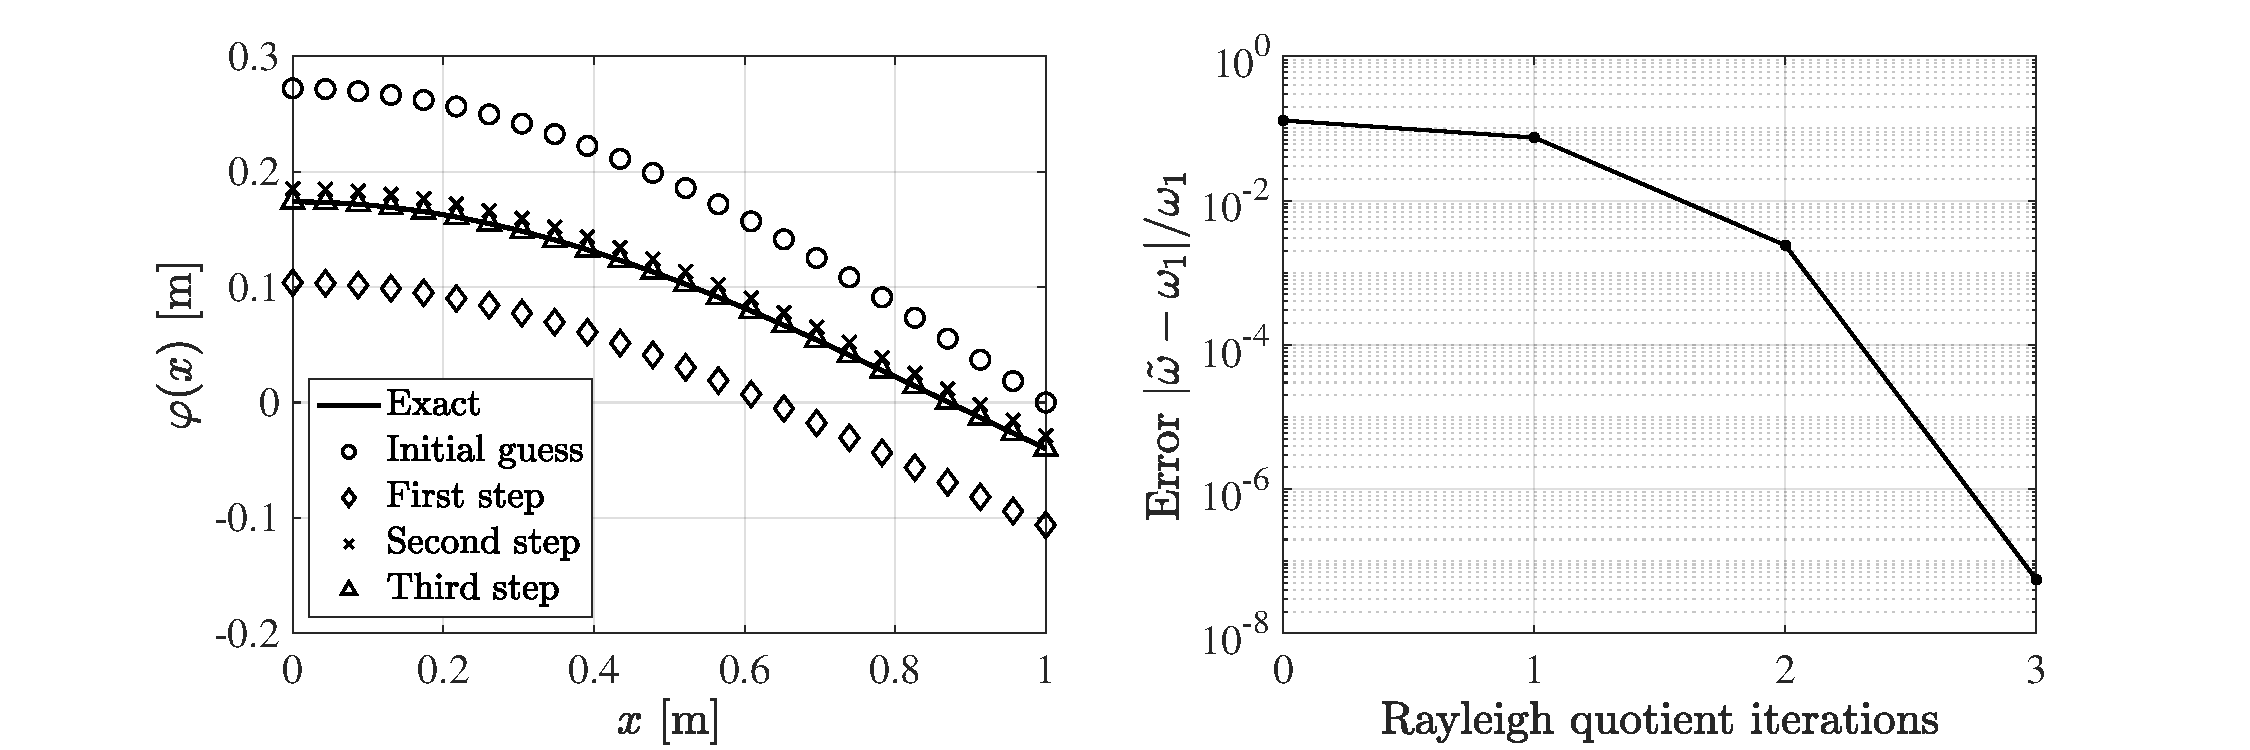
\includegraphics[width=\textwidth]{homework/hw3/assets/hw3_p5_results.pdf}
        \caption{Rayleigh quotient iteration (3 steps) convergence of the first eigenfunction (left) and eigenvalue (right), compared with the exact value computed in part (i). }
        \label{fig:hw3_p5_results}
    \end{figure}
    
}
\end{enumerate}

\begin{problem}
    \textbf{6 (100 points)}. Prove Rayleigh's principle: 
    If a trial function is $\order{\epsilon}$ close to the eigenfunction $\varphi_r(x)$, i.e., $\varphi(x) = \varphi_r(x) + \sum_{i=1, i\neq r}^\infty \epsilon_i \varphi_i(x)$, $\epsilon_i = \order{\epsilon}, ~0 < \epsilon \ll 1$, then the estimate for the $r$-th natural frequency obtained from Rayleigh's quotient can be expressed as 
    \begin{equation}\label{eqn:hw3_p6_rayleigh_principle}
        \omega^2 = R[\varphi(x)] = \omega_r^2 + \sum_{i=1}^{\infty} (\omega_i^2 - \omega_r^2) \epsilon_i^2
    \end{equation}
    where $\omega_i$ is the $i$-th natural frequency of the system.
\end{problem}
An underlying eigenvalue problem for the statement above is as follows: 
\begin{subequations}\label{eqn:hw3_p6_eigenproblem}
\begin{align}
    \frac{d}{dx} \left[A(x) \frac{d\varphi}{dx}(x) \right] + \omega^2 B(x) \varphi(x) &= 0, \\
    A(0) \frac{d\varphi}{dx}(0) - (k_1 - \omega^2 M_1) \varphi(0) &= 0, \\
    A(L) \frac{d\varphi}{dx}(L) + (k_2 - \omega^2 M_2) \varphi(L) &= 0.
\end{align}
\end{subequations}
Given an \emph{admissable} trial function $\varphi(x)$, its generalized Rayleigh quotient associated with this problem reads 
\begin{equation}\label{eqn:hw3_p6_rayleigh_quotient}
    \omega^2 \approx R[\varphi(x)] = \frac{K_1\varphi^2(0) + K_2 \varphi^2(L) + \int_0^L A(x) {\varphi'(x)}^2 dx}{M_1\varphi^2(0) + M_2 \varphi^2(L) + \int_0^L B(x) {\varphi(x)}^2 dx}.
\end{equation}
Let $\varphi_i(x), i = 1, 2, \ldots$ be the $i$-th eigenfunction and $\omega_i$ the $i$-th eigenvalue. 
One can establish the mass and stiffness ortho-normality conditions from \cref{eqn:hw3_p6_eigenproblem} as (shown in lecture)
\begin{subequations}\label{eqn:hw3_p6_orthonormality}
\begin{align}
    M_1\varphi_i(0) \varphi_j(0) + M_2\varphi_i(L) \varphi_j(L) + \int_0^L B(x) \varphi_i(x) \varphi_j(x) dx &= \delta_{ij}, \\
    K_1\varphi_i(0) \varphi_j(0) + K_2\varphi_i(L) \varphi_j(L) + \int_0^L A(x) \varphi_i'(x) \varphi_j'(x) dx &= \omega_i^2 \delta_{ij}.
\end{align}
\end{subequations}
For convenience, we rewrite the decomposition of $\varphi(x)$ as 
\begin{equation}\label{eqn:hw3_p6_decomp}
    \varphi(x) = \sum_{i=1}^\infty \mu_i \varphi_i(x), ~~~~ \mu_i = \begin{cases}
        \epsilon_i = \epsilon \eta_i, & i \neq r, \\
        1, & i = r.
    \end{cases}
\end{equation}
where $\eta_i = \order{1}$.
Substituting \cref{eqn:hw3_p6_decomp} into \cref{eqn:hw3_p6_rayleigh_quotient} leads to
\begin{equation}
\begin{aligned}
    R[\varphi(x)] &= \frac{
        K_1 \sum_{i,j=1}^\infty \mu_i\mu_j\varphi_i(0)\varphi_j(0) + K_2 \sum_{i,j=1}^\infty \mu_i\mu_j\varphi_i(L)\varphi_j(L) + \int_0^L A(x) \sum_{i,j=1}^\infty \mu_i\mu_j\varphi_i'(x) \varphi_j'(x) dx
    }{
        M_1 \sum_{i,j=1}^\infty \mu_i\mu_j\varphi_i(0)\varphi_j(0) + M_2 \sum_{i,j=1}^\infty \mu_i\mu_j\varphi_i(L)\varphi_j(L) + \int_0^L B(x) \sum_{i,j=1}^\infty \mu_i\mu_j\varphi_i(x) \varphi_j(x) dx
    } \\
    &= \frac{
        \sum_{i,j=1}^\infty \mu_i \mu_j \left[ K_1\varphi_i(0) \varphi_j(0) + K_2\varphi_i(L) \varphi_j(L) + \int_0^L A(x) \varphi_i'(x) \varphi_j'(x) dx \right]
    }{
        \sum_{i,j=1}^\infty \mu_i \mu_j \left[ M_1\varphi_i(0) \varphi_j(0) + M_2\varphi_i(L) \varphi_j(L) + \int_0^L B(x) \varphi_i(x) \varphi_j(x) dx \right]
    } \\
    &= \frac{
        \sum_{i,j=1}^\infty \mu_i \mu_j \omega_i^2 \delta_{ij}
    }{
        \sum_{i,j=1}^\infty \mu_i \mu_j \delta_{ij}
    } \\
    &= \frac{\sum_{i=1}^\infty \mu_i^2 \omega_i^2}{\sum_{i=1}^\infty \mu_i^2} = \frac{\omega_r^2 + \epsilon^2\sum_{i=1, i\neq r}^\infty \eta_i^2 \omega_i^2}{1 + \epsilon^2 \sum_{i=1}^\infty \eta_i^2}.
\end{aligned}
\end{equation}
where we have leveraged the ortho-normality conditions \cref{eqn:hw3_p6_orthonormality}.
Note also that asymptotically, $1 / (1 + \epsilon \eta) = 1 - \epsilon \eta + \order{\epsilon^2}$.
Hence, the Rayleigh quotient can be further expanded as 
\begin{equation}
\begin{aligned}
    R[\varphi(x)] &= \left(\omega_r^2 + \epsilon^2 \sum_{\substack{i=1, \\ i\neq r}}^\infty \eta_i^2 \omega_i^2\right) \left(1 - \epsilon^2 \sum_{i=1}^\infty \eta_i^2 + \order{\epsilon^4} \right) \\
    &= \omega_r^2 + \epsilon^2 \sum_{i=1}^\infty \eta_i^2 (\omega_i^2 - \omega_r^2) + \order{\epsilon^4}.
\end{aligned}
\end{equation}
where the $i\neq r$ subscript is not needed as $\omega_i^2 - \omega_r^2 = 0$ when $i = r$.
By dropping higher order terms and substituting $\epsilon_i = \epsilon \eta_i$, we recover Rayleigh's principle \cref{eqn:hw3_p6_rayleigh_principle}.
